\documentclass[12pt,letterpaper]{article}
\usepackage[parfill]{parskip}
\usepackage{graphicx}
\graphicspath{ {./images/} }

\begin{document}

\section*{CptS 453 | Homework-03 }
\subsection*{Charles Nguyen, \#011606177 }

\subsection*{Problem 1:}


The bijection is $\psi: V_i \rightarrow U_i $, where:
\[ V = \{0,1,2,3,4,5,6,7,8,9\} \]
\[ U = \{a,d,j,e,b,c,i,g,h,f\} \]
are both order sets.

\subsection*{Problem 2:}

For:

- $P_a: a - 1$

- $C_a: a - 1$

- $K_a: a - 1$

- $K_{a,b}: 2a - 1, \mbox{ where } a \leq b$

- $Q_a: a - 1$

\subsection*{Problem 3:}


\pagebreak
\subsection*{Problem 4:}

\subsubsection*{A.}

In terms of $|V_G|$ and $|V_H|$, $|V_{G {\times} H}| = |V_G| \cdot |V_H|$.

\subsubsection*{b.}
Given the proof above, in order for a cubic graph of order $n=4$ to exist, we
can see right away that the degree $k=n-1=3$. Thus the number of edges in the
graph will be $\frac{nk}{2} = 6$. The following image shows such a graph:

\begin{figure}[h]
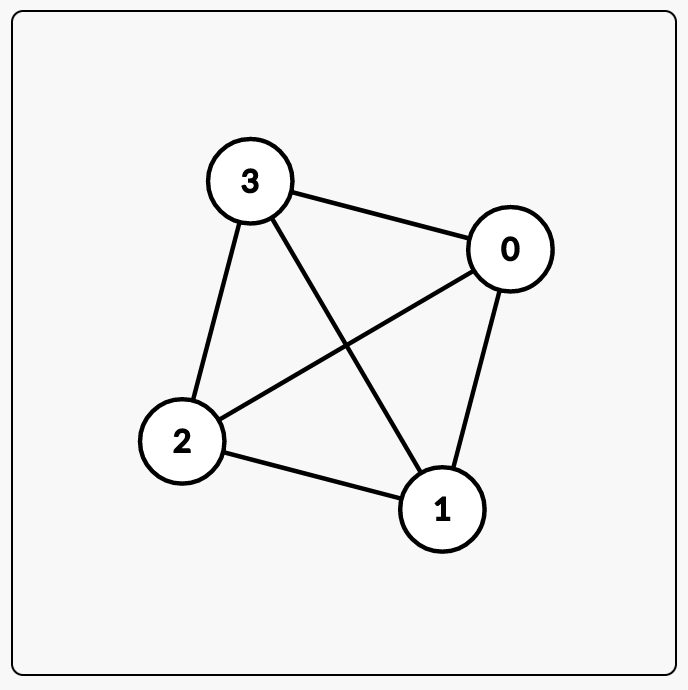
\includegraphics[scale=0.20]{n4k3}
\centering
\end{figure}

\subsubsection*{c.}
Given input $V$ of order $2n$, we can decompose $V$ into $V_1$ of order $n$
and $V_2$ of the same order $n$.  This allows us to construct a \emph{biparte} graph of degree $k=n$.

\end{document}
